\documentclass{article}
\usepackage[margin=1in]{geometry}
\usepackage{amsmath}
\usepackage{amssymb}
\usepackage{graphicx}

\begin{document}
\begin{titlepage}
   \vspace*{\stretch{1.0}}
   \begin{center}
      \Large\textbf{Determining Robot Position Relative to Vision Target by Analyzing Camera Image}\\
      \large\textit{Author: Peter Stoeckl}\\
      \large\textit{Revised by: Andrew Messing}
   \end{center}
   \vspace*{\stretch{2.0}}
\end{titlepage}

\begin{abstract}
Using the FRC Camera in conjunction with the NI Vision software, the robot’s position relative to a vision target can be determined. The Vision software can detect ellipses in the camera image and measure their major and minor diameters. The ellipse detection software can thus measure the apparent deformation of the target by the camera’s changing angle relative to the target, which can be used to determine the robot’s position. 
\end{abstract}

First, it is necessary to examine the relation between the camera image and the target’s dimensions.

		\begin{figure}[!htbp]

		\centering

		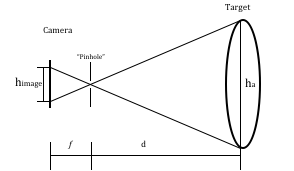
\includegraphics{pinhole_model.png}

		\end{figure}

Assuming the camera to be equivalent to a pinhole camera makes it easy to see that the height himage of the target on the camera image and the effective focal length $f$ of the camera are proportional to the target’s apparent actual height (see below) $h_{a}$ and the distance $d$ from the camera to the target: $$\frac{h_{image}}{f} = \frac{h_{a}}{d}$$  The same applies to the respective widths: $$\frac{w_{image}}{f} = \frac{w_{a}}{d}$$

\begin{figure}[!htbp]

		\centering

		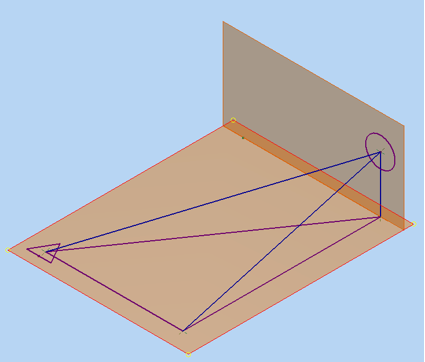
\includegraphics{3d_target_model.png}

		\caption{Diagram of the target as viewed by the camera}

\end{figure}

\begin{figure}[!htbp]

		\centering

		
\includegraphics{yz_target_model.png}

\end{figure}

The vision target has a true diameter (thus height) $h_{0}$, which is known. The difference in elevation $z$ between the camera and the center of the target is also known. The camera’s (effective) focal length $f$ can be determined by experimentation. At a constant horizontal distance $d_{h}$ from the target, the height of the target on the image ($h_{image}$) remains constant. This value can be determined using the ellipse detection software. The camera is not detecting the true height of the target, however, but instead an apparent height $h_{a}$; the plane of this apparent height is at an angle of $\alpha$ to the vertical, which can be shown to be the same as the angle between the line from the camera to the center of the target (with length $d$) and the horizontal.

Then $d$ is the distance from the camera to the target, and since $sin(\alpha) = \frac{z}{d}$, $d = \frac{z}{sin(\alpha)}$. Also, since the angle between the two h planes is $\alpha$, $h_a = h_0 * cos(\alpha)$. Substituting these values into $\frac{h_{image}}{f} = \frac{h_a}{d}$ yields $\frac{h_{image}}{f} = \frac{(h_0 cos(\alpha) sin(\alpha))}{z}$. $cos(\alpha)sin(\alpha) = \frac{1}{2} sin(2 \alpha)$, therefore $\frac{h_{image}}{f} = \frac{(h_0 sin(2 \alpha))}{2z}$. Solving for $\alpha$ yields $\alpha = \frac{asin (\frac{(2zh_{image})}{fh_0})}{2}$. Then $tan(\alpha) = \frac{z}{d_h}$, therefore  $d_h = \frac{z}{tan(\alpha)}$. Thus the horizontal straight-line distance, $d_h$,  from the robot (with the camera) to the target can be determined.

\begin{figure}[!htbp]

		\centering

		
\includegraphics{xy_target_model.png}

\end{figure}

From the first section, $\frac{w_{image}}{f} = \frac{w_{a}}{d}$, therefore $ w_a = \frac{dw_{image}}{f}$. Also (by the same argument as in the second section) $w_a = w_0 cos(\beta)$, $w_0$ being equal to $h_0$ since the target is circular. Substituting, $w_0 cos(\beta) = \frac{dw_{image}}{f}$, and then solving for $\beta$: $\beta = acos (\frac{dw_{image}}{fw_0})$. (Note that $d = \frac{z}{sin(\alpha)}$—see previous section). This is, however, not in a horizontal position (see 3-D diagram); the true horizontal angle $\beta_h$ is therefore different from $\beta$. The length $y = d sin(\beta)$, and $d_h = d cos(\alpha)$; then $sin(\beta_h) = \frac{y}{d_h} = \frac{d sin(\beta)}{d cos(\alpha)} = \frac{sin(\beta)}{cos(\alpha)}$, and therefore $\beta_h = asin (sin(\beta) ÷ cos(\alpha))$ . The angle of the robot (and camera) from the target has now been determined. In addition, it is now possible to locate the robot with cartesian coordinates relative to the target; the distance in one direction (y) has already been calculated; in the other direction, $x = d_h sin(\beta_h)$.

Final Note: This algorithm does not give enough information to determine whether the robot is $\beta_h$ degrees to the left or to the right of the target. However, if it is known which target on the Breakaway field is being observed, this can be determined to a reasonable degree of certainty. Since the targets are very close to the sides of the field, it is very unlikely that the camera will be on the side of the target nearer the side of the field; therefore the robot will most likely be to the left of the targets labeled L below and to the right of the targets labeled R.

\end{document}